\section{Introdução}

Um compilador é composto por duas partes principais: o \textit{front end} e o \textit{back end}. O \textit{front end} analisa o código fonte a fim de construir uma representação interna do programa, chamada de representação intermediária. Para tal ele se utiliza de uma estrutura de dados chamada tabela de símbolos, a qual será passada adiante junto com a representação gerada. Já o \textit{back end} trata da construção do programa objeto a partir da representação intermediária e da tabela de símbolos, realizando otimizações no código, quando possível.

O trabalho em questão tem como objetivo implementar o \textit{front end} de um compilador, cujas fases estão destacadas na Figura \ref{fig:front_end}, para a linguagem \textbf{SmallL}. Essa linguagem é descrita pela gramática apresentada na Figura \ref{fig:grammar}. Para codificação dos componentes do compilador se utilizou a linguagem de programação \textbf{Java} (\textit{v.8}). 

O trabalho foi desenvolvido utilizando a ferramenta de versionamento Git juntamente com a plataforma de desenvolvimento remoto GitHub. O repositório do projeto contém não só o código fonte, mas também os scripts auxiliares desenvolvidos e os arquivos de teste, podendo ser acessado no endereço \url{https://github.com/joaofbsm/smallL}.

\begin{figure}[H]
 	\centering
	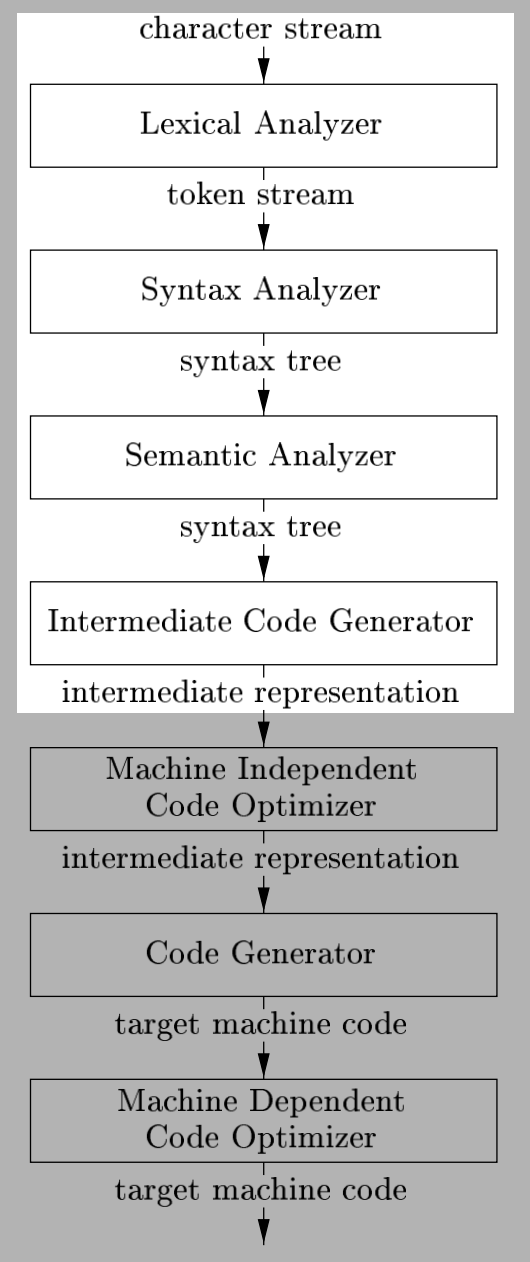
\includegraphics[width=6cm,keepaspectratio]{imgs/front_end.png}
	\caption{Componentes do \textit{front end} de um compilador (destacados em branco)}.
	\label{fig:front_end}
\end{figure}

\begin{figure}[H]
 	\centering
	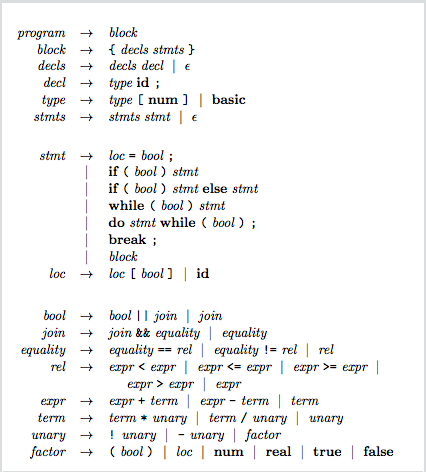
\includegraphics[width=1\textwidth]{imgs/grammar.png}
	\caption{Gramática inicial que descreve a linguagem \textbf{SmallL}}.
	\label{fig:grammar}
\end{figure}